\section*{Capítulo 03: Governança de relações contratuais}

Em linhas gerais, ECT estabelece que a variedade de instituições está associada com os atributos das \textbf{transações} e que o propósito de eficiência das instituições diz respeito à combinação da estrutura de governança adequada aos atributos mencionados. Dito isso, neste capítulo, Williamson analisa as diferentes teorias e abordagens dos contratos.

\subsection*{Tradições contratuais}

O autor argumenta que o paradigma da \textbf{transação discreta} é difundido tanto em direito quanto em economia, mas há o reconhecimento que muitas relações contratuais não podem ser configuradas enquanto discretas.

\begin{description}
	\item[Clássica] Enfatiza o caráter discreto e presencial (``\textit{presentation}'') dos contratos. Implica irrelevância das partes contratuais e destaca em regras formas;
	\item[Neo-clássica] Parte do reconhecimento de que o mundo é um sistema complexo e que os contratos são incompletos por consequência e que as partes irão cumpri-los a depender da confiança no aparato jurídico associado;
	\item[Relacional] A impessoalidade da teoria clássica é descartada e dá lugar a um tratamento relacional ao longo do tempo em que a especificidade das transações se destacam
\end{description}


\begin{figure}[h]
	\centering
	\caption{Transações ilustrativas}
	\label{fig:screenshot006}
	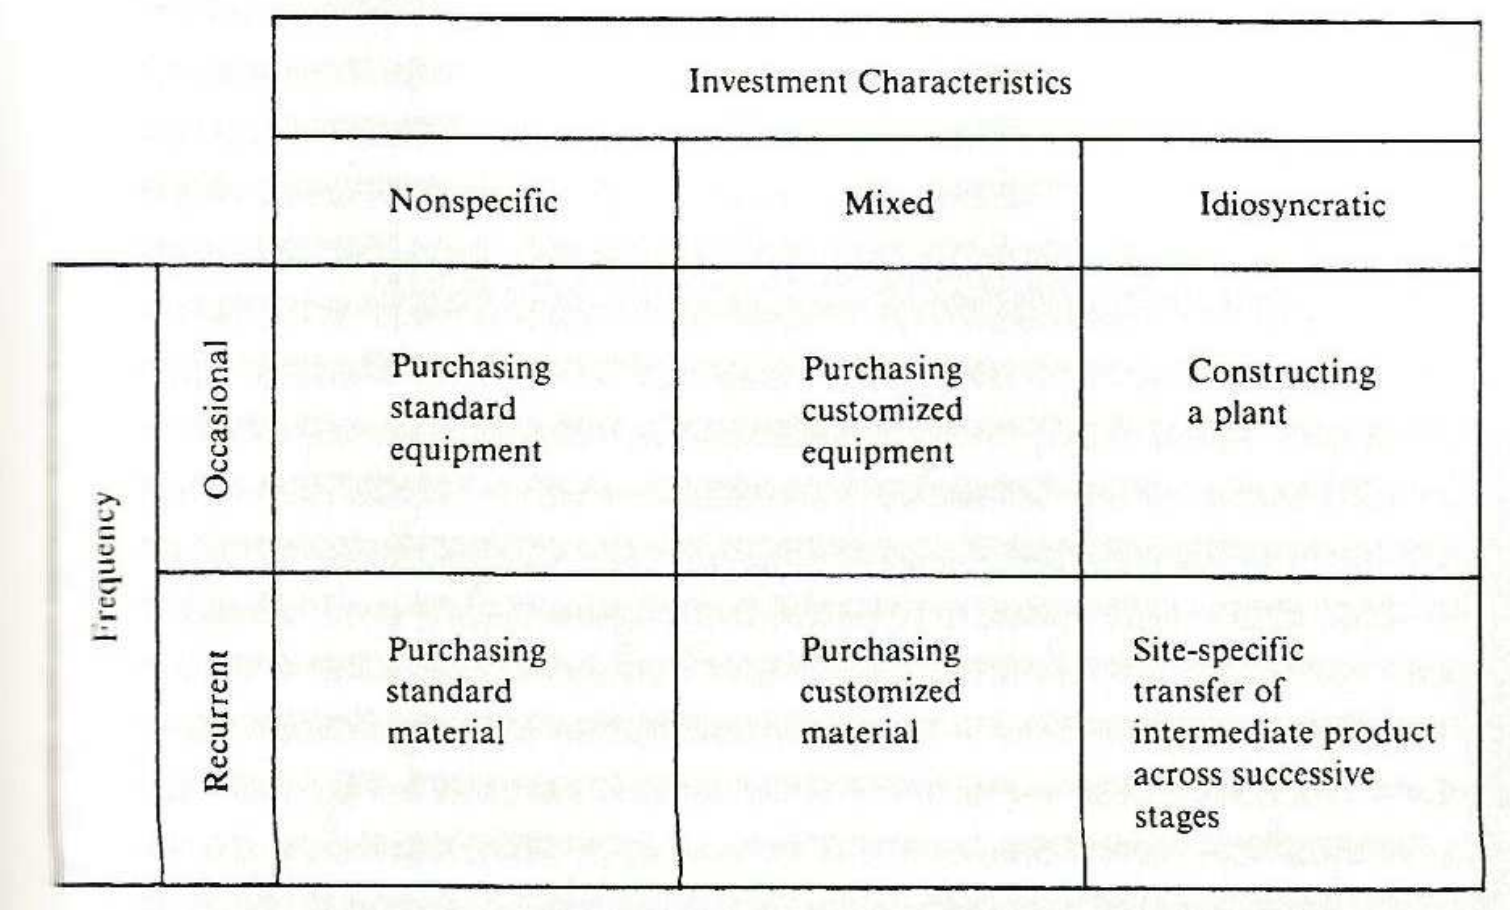
\includegraphics[width=0.7\linewidth]{screenshot006}
\end{figure}



\subsection*{Governanças eficientes}

Apesar das transações terem outras dimensões, Williamson irá focar na especificidade dos ativos e na frequência categorizados da seguinte maneira e sintetizados na tabela abaixo:

\begin{itemize}
	\item Frequência
	\begin{itemize}
		\item Única
		\item Ocasional
		\item Recorrente
	\end{itemize}
	\item Especificidade dos ativos
	\begin{itemize}
		\item Não-específicos
		\item Mistos
		\item Altamente específicos
	\end{itemize}
	\item Hipóteses simplificadoras
	\begin{itemize}
		\item Firmas temporárias podem ser desconsideradas
		\item Ofertantes potenciais são numerosos
		\item Frequência diz respeito à atividade de compra no mercado somente
		\item $\therefore$ Apenas transações ocasionais e frequentes serão consideradas e a especificidade da governança está diretamente associada tanto com a frequência quanto com a especificidade do ativo em questão
	\end{itemize}
\end{itemize}

\begin{figure}[h]
	\centering
	\caption{Governanças eficientes}
	\label{fig:screenshot007}
	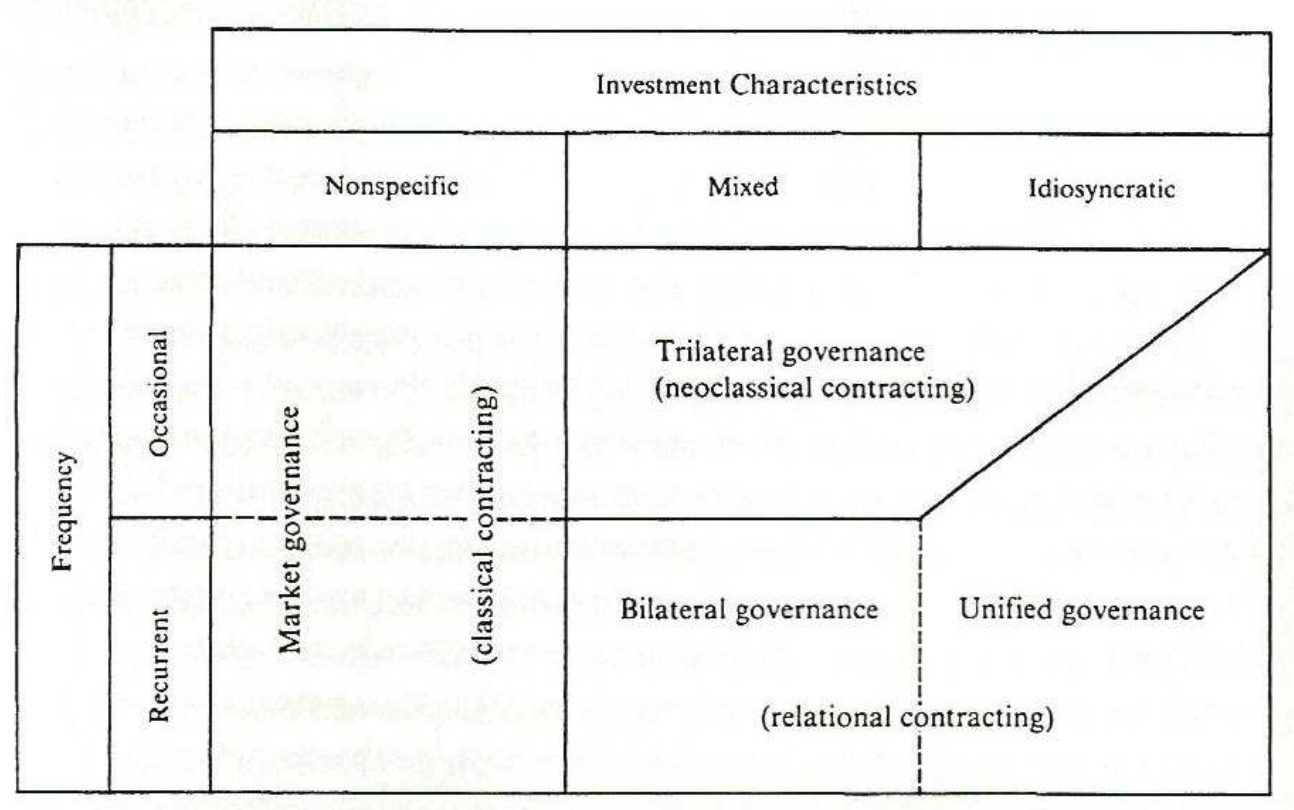
\includegraphics[width=0.7\linewidth]{screenshot007}
\end{figure}




\begin{description}
	\item[Mercado:] É a principal estrutura de governança para transações \textbf{não-específicas}, sejam elas ocasionais ou frequentes. Este tipo de transação é aquele que os contratantes estão menos aptos a se basear em suas experiências para estabelecer salvaguardar contra o comportamento oportunista. Em linhas gerais, as implicações do paradigma discreto se aplicam a esta estrutura de governança. A identidade das partes é negligenciável e o conteúdo das transações está sujeito à formalidades;
	\item[Trilateral:] São mais necessárias em transações ocasionais em que a especificidade é mista ou elevada. Sendo assim, não existem incentivos suficientes para que o contrato se dê via competição, ou seja, o mercado é insuficiente.
	\item[Bilateral:] São mais frequentes em transações frequentes cuja especificidade dos ativos é média ou elevada. Como consequência, a \textbf{transformação fundamental} ocorre por conta da natureza não convencional/padronizada das transações. Além disso, a recorrência das transações faz com que os custos elevados de uma governança especializada seja diluído. Além disso, tais estruturas preservam a \textbf{autonomia} das partes, seja pela verticalização ou relação entre-firmas. Ambas as partes têm incentivos para preservas as relações contratuais.
	\item[Unificada:] Os incentivos para as relações entre-firmas se reduzem na medida que as transações se tornam progressivamente mais específicas, ou seja, menos transferível para o uso de outros sem perdas significativas de modo que as economias de escala são realizadas por uma das partes (verticalização). A vantagem da verticalização é a menor necessidade de revisão dos contratos entre-firmas.
\end{description}

\subsection*{Incerteza}

A presença da incerteza impõe uma problema adaptativo e sequencial. Em linhas gerais, um maior grau de incerteza não afeta significativamente as transações de ativos menos específicos. No entanto, quanto maior a \textbf{especificidade dos ativos} e dada a necessidade de \textbf{continuidade} das relações contratuais, a incerteza se torna mais impositiva de modo que estruturas de governança mais adequadas são necessárias. Uma forma de lidar com a incerteza é optar por ativos menos específicos e mais usuais de modo que a governança de mercado é mais adequada. No entanto, tal especificidade pode ser preservada com uma forma de organização internalizada.

\subsection*{Mensuração}

Em linhas gerais, Williamson pontua que os problemas de governança e mensuração (ambos ramos da ECT) são negligenciáveis na ausência \textbf{tanto} de racionalidade ilimitada \textbf{quanto} de comportamento oportunista. Na ausência de racionalidade limitada, os custos de mensuração são nulos em que o comportamento oportunista invalidado. Na ausência de comportamento oportunista, a incompletude dos contratos deixa de ser um problema de governança.


\subsection*{Distribuição das transações}

Nesta seção, Williamson discute qual a ``distribuição de frequência'' dos diferentes tipos de contrato e transações. Conclui que uma distribuição \textbf{uniforme} é a que melhor descreve o mundo contratual.